\documentclass[11pt]{article}
\usepackage[margin=2.5cm]{geometry}
\usepackage{amsmath, amssymb}
\usepackage{graphicx}
\usepackage{hyperref}
\usepackage{siunitx}
\usepackage{enumitem}
\usepackage{fancyhdr}
\usepackage{booktabs}
\usepackage{xcolor}
\pagestyle{fancy}
\fancyhf{}
\lhead{Computational Physics – Project Brief}
\rhead{Department of Physics, Lund University}
\cfoot{\thepage}
\definecolor{mygrey}{gray}{.85}
\renewcommand{\headrulewidth}{0.4pt}
\newcommand{\exercise}[1]{\par \vspace{0.5cm} \noindent  {\large \colorbox{mygrey}{\begin{minipage}{\textwidth}{\textbf{Math exercise}}\end{minipage}}} \par \noindent \begin{quote} 
\small{#1} \\
\footnotesize{\textit{Math exercises are \textbf{not mandatory}, but useful to get more familiar with the derivations. Do the Simulation tasks first.}}
\end{quote} 
\begin{tabular}{c} \\ \toprule \\ \hspace{15cm} \\ \end{tabular}}
\begin{document}

\begin{center}
  {\Large \textbf{Project: Entropic spring -- rediscover Hooke's law with Monte Carlo}}\\[6pt]
  {\large MC sampling, statistical physics, reweighting, scientific visualization}\\[4pt]
  {Christian Bierlich, Department of Physics, Lund University,}\\
  {E-mail: \texttt{christian.bierlich@fysik.lu.se}}
\end{center}

\vspace{0.75em}

\noindent\textbf{Summary.}
You will build a simulation of rubber bands, being pulled by a force, in 1 dimension. You will calculate basic observables (``how stretched is the rubber band?'') as function of force in two ways: 1) by reweighting, and 2) by direct simulation.

This exercise will \emph{not} provide you with a large amount of template code to start with. Rather, it is up to you, to set up reasonable data structures etc. for this project.

The main goal of this exercise is to familiarize you with Monte Carlo methods. You should therefore \emph{not} rely on library implementations of Monte Carlo selection apart from sampling a random number in the interval $R \in [0,1]$
\medskip

\noindent\textbf{Learning goals.}
When you have completed this exercise, you will be able to:
\begin{itemize}
  \item Translate a simple physical model (the entropic spring) into a working computational simulation using object-oriented programming.
  \item Apply Monte Carlo sampling techniques to generate and analyze ensembles of microstates, including the use of weighted (reweighted) samples.
  \item Quantitatively compare Monte Carlo results to analytical predictions, using ratio plots and statistical measures to validate simulations.
  \item Diagnose and interpret the performance and limitations of Monte Carlo methods, including ensemble overlap and effective sample size.
\end{itemize}

\section*{Physics background}
We consider a simple model of a rubber band in one dimension. A chain consisting of $N \gg 1$ links, each of length $a$. For simplicity, we will assume that all configurations of the chain have the same energy, all that matters for the properties of the chain is how many times it doubles back on itself.
We will thus have a number of links pointing in the $+$-direction, and the rest pointing in the $-$-direction. If we call the total length of the chain $L$, and the number of links pointing in the $+$-direction $n$, we have:
\begin{equation}
\label{eq:L-def}
L = a(2n - N).
\end{equation}
We know from basic thermodynamics, the relation between entropy ($S$) and force ($f$) at fixed energy ($E$) to be:
\begin{equation}
  \vec{f} = -T\left( \frac{\partial S}{\partial \vec{x}} \right)_E,
\end{equation}
at temperature $T$ with $\vec{x}$ being the spatial extension\footnote{Note: $\vec{x}$ may be more familiar from the definition of work: $dW = \vec{f}d\vec{x}$: work is equal to force times path.}. We reduce to one dimension for simplicity:
\begin{equation}
\label{eq:force-1d}
  f = -T\left( \frac{\partial S}{\partial L} \right)_E,
\end{equation}
and our task is now to calculate the microscopic entropy, and see how it changes with $L$.

\begin{figure}
  \begin{center}
  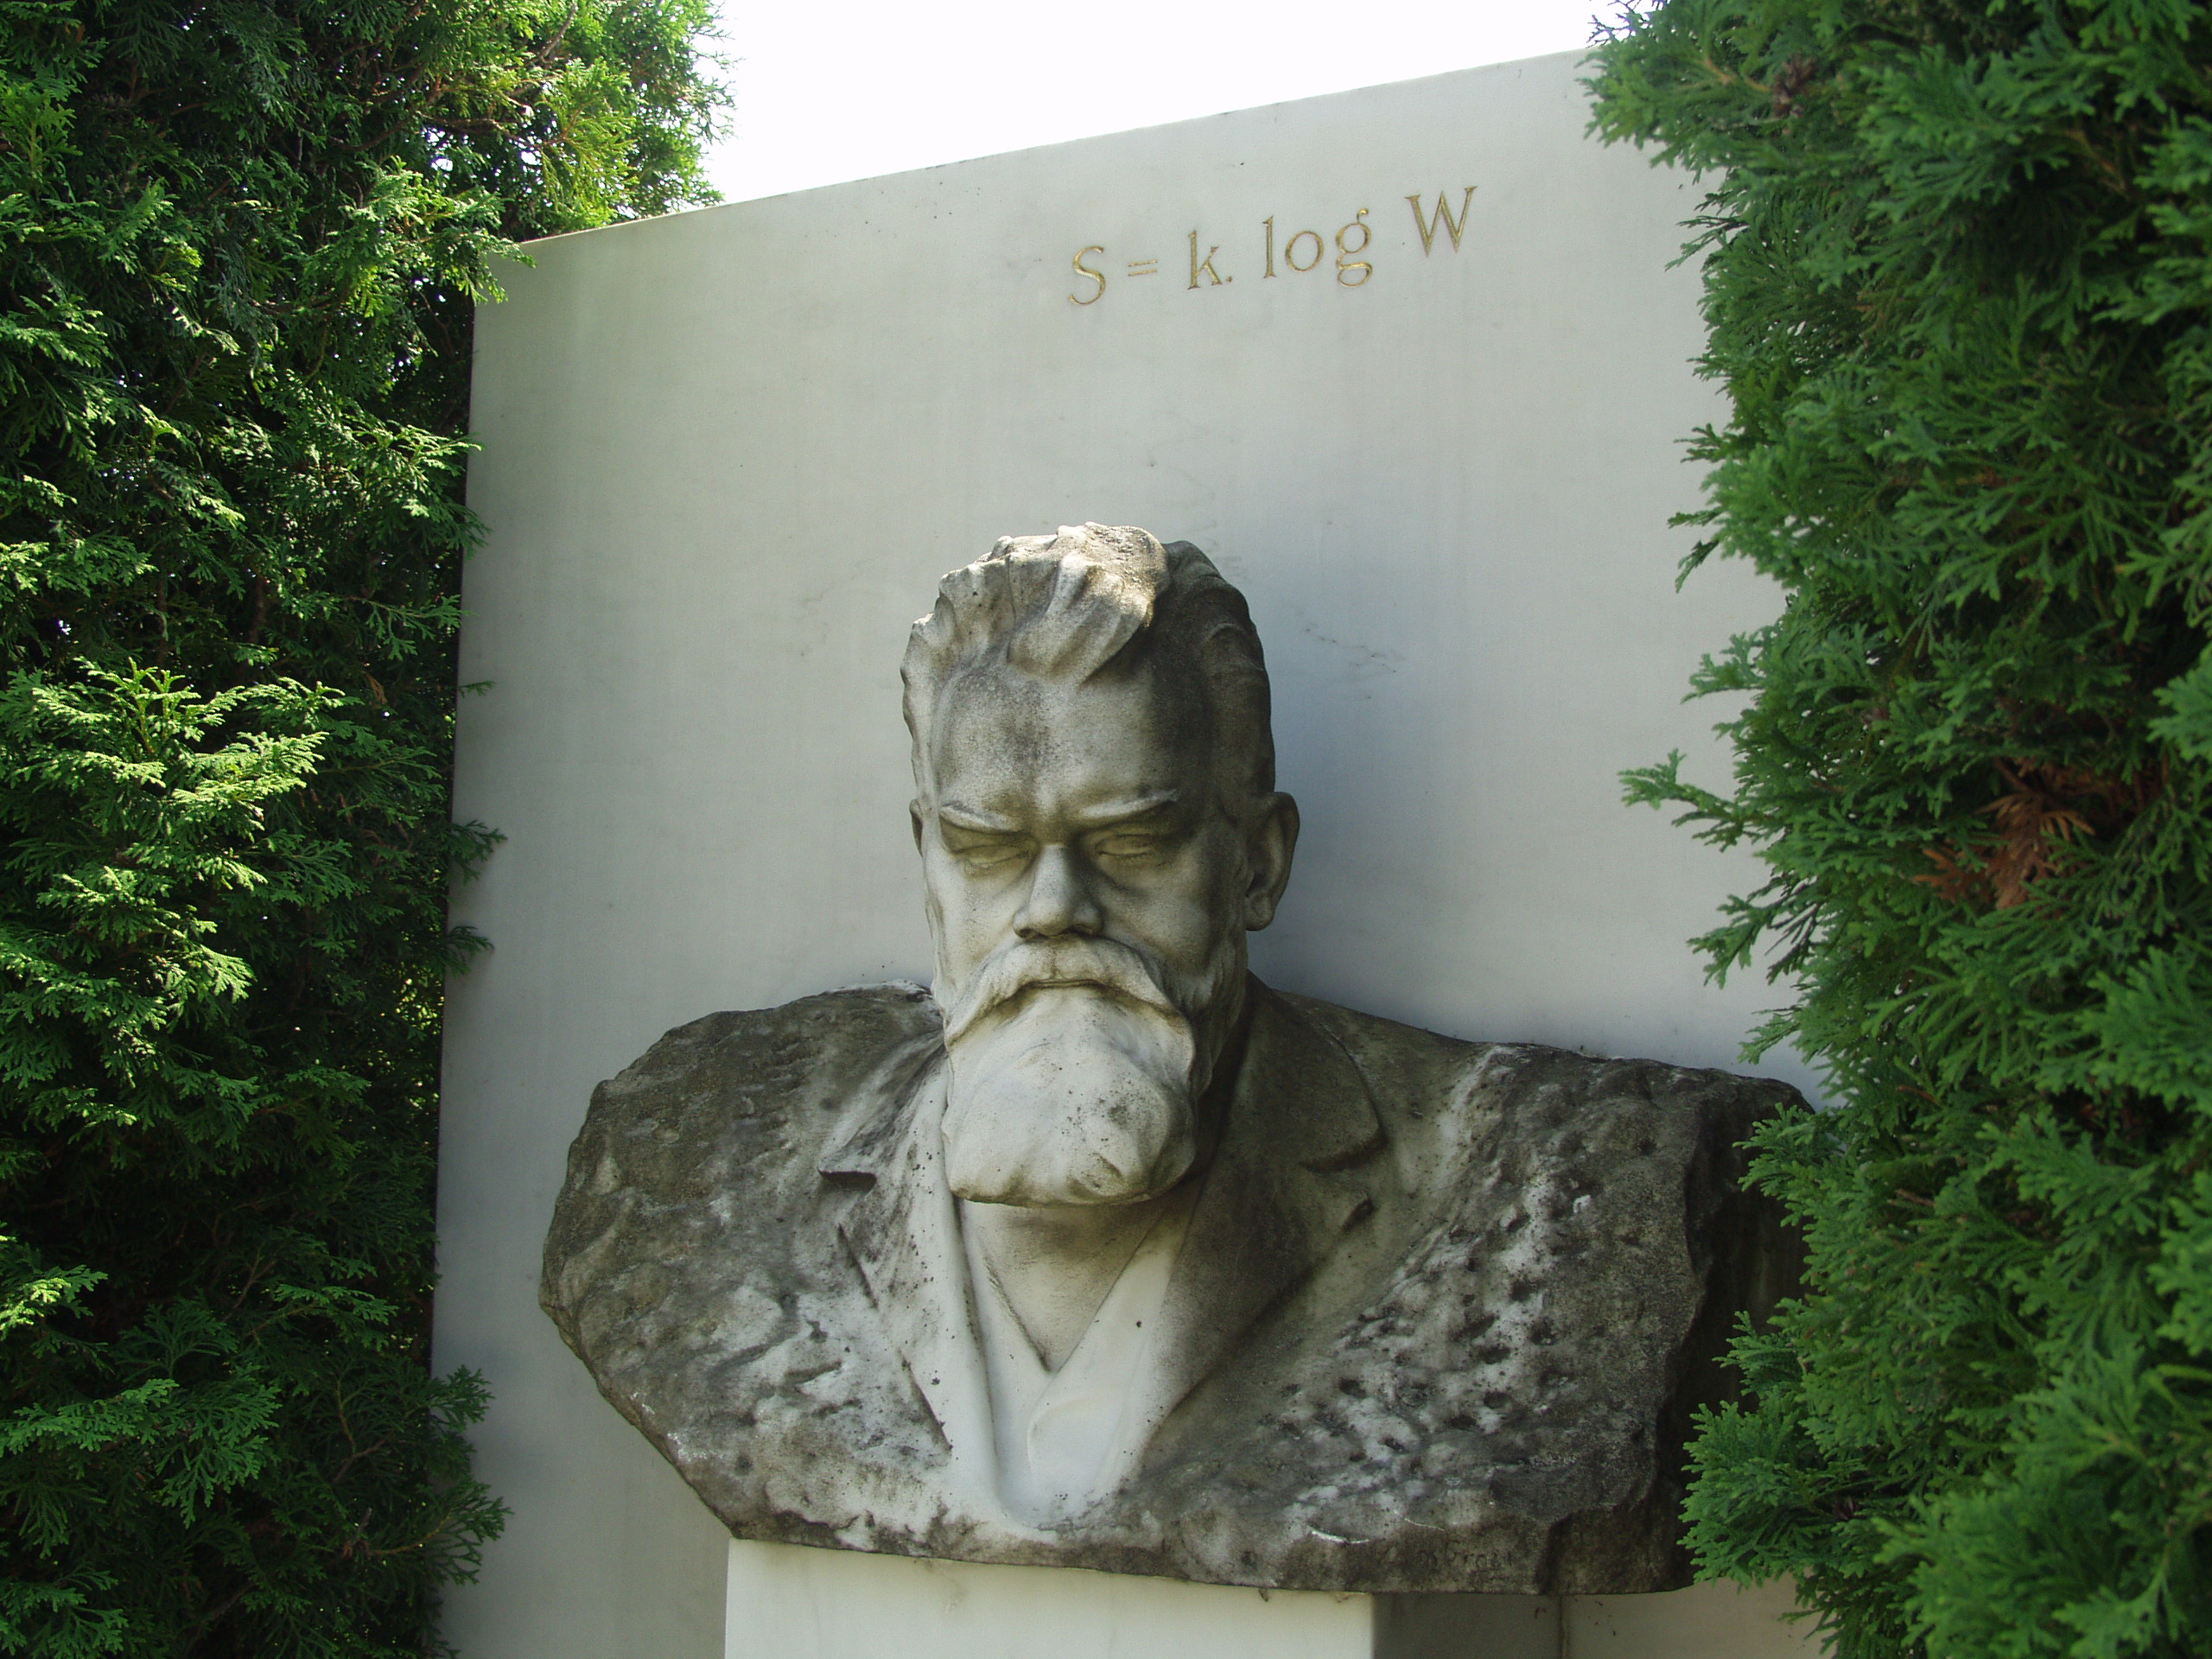
\includegraphics[width=0.8\textwidth]{boltzmann-grave.jpg}
  \end{center}
  \caption{\label{fig:boltzmann}Ludwig Boltzmann (1844–1906), Austrian physicist and one of the founders of statistical mechanics. He established the microscopic interpretation of entropy, relating it to the number of accessible microstates through eq. \eqref{eq:entropy-def} This relation is famously engraved on his tombstone in Vienna’s Zentralfriedhof cemetery, as seen in the picture (Credit: \href{http://users.fred.net/tds/lab/images/boltzmann/}{Thomas D. Schneider, MIT}).
  Boltzmann’s work laid the foundation for modern thermodynamics, kinetic theory, and statistical physics.}
\end{figure}

From Boltzmann's tombstone (see fig. \ref{fig:boltzmann}), we know that the entropy counts the number of microstates corresponds to a given macrostate ($\Omega$):
\begin{equation}
\label{eq:entropy-def}
  S = k_B\ln(\Omega),
\end{equation}
with $k_B$ being Boltzmann's constant. A macrostate is specified by the total extension $L$. Many microstates (different orderings of $\pm$ links) correspond to the same $L$. 

The number of ways to arrange the chain such that $n$ links point in the positive direction, is given by the Binomial coefficient:
\begin{equation}
  \Omega(N,n) = \binom{N}{n} = \frac{N!}{n!(N-n)!}.
\end{equation}
Using Stirling's approximation\footnote{Which states that $\ln(n!) \approx n \ln(n) - n$ when $n$ is large.} we get:
\begin{equation}
\frac{S}{k_B} \approx N\ln(2) - \frac{L^2}{2Na^2}.
\end{equation}

\exercise{
Fill in the remaining steps of algebra in this derivation. (Hint: First you must apply Stirling's approximation. This gives you two logarithms, which you can Taylor expand in $L/(Na)$ which is always smaller than unity.)
}

Inserting in eq. \eqref{eq:force-1d}, gives directly:

\begin{equation}
\label{eq:hookes-law}
  f = \frac{k_B T }{Na^2} L.
\end{equation}

Comparing to Hooke's law: $f = kL$, we identify an entropic spring constant $k = k_B T / (Na^2)$.

\section*{Simulation tasks}

\subsection*{Simulation task I: microstates and macrostates} Consider first an ensemble of unbiased microstates. That is, rubber bands which we are not pulling with any force, they are just random configurations.
\begin{itemize}
  \item Set up reasonable data structures, a \texttt{Link} class and a \texttt{RubberBand} class both holding relevant parameters. The \texttt{RubberBand} class should have a method which calculates the total length $L$. The constructor of \texttt{RubberBand} should take $N$ as a parameter, and randomly sample \texttt{Link}s pointing in $+$ -or $-$ direction, and store them as a data member.
  \item Monte Carlo sample a large number of rubber bands. Let $a = 1$ for simplicity, and let $N=100$.
  \item Make a histogram of the $P(L)$-distribution. Compare to the analytic result: $P(L) = \Omega(N,n)/2^N$ (remember: $\Omega$ is the number of microstates with extension $L$, $2^N$ is the total number of microstates. The ratio is the probability.)
  \item Your comparison should (at least) consist of plotting the two overlaid with each other, a plot of the ratio of the two (unity means identical) and some sort of quantitative measure, such as $\chi^2/$ndf. In figure \ref{fig:demo-fig} you can see what the figure should look like, with inspiration for how to plot and present it. 
\end{itemize}

\begin{figure}
\begin{center}
  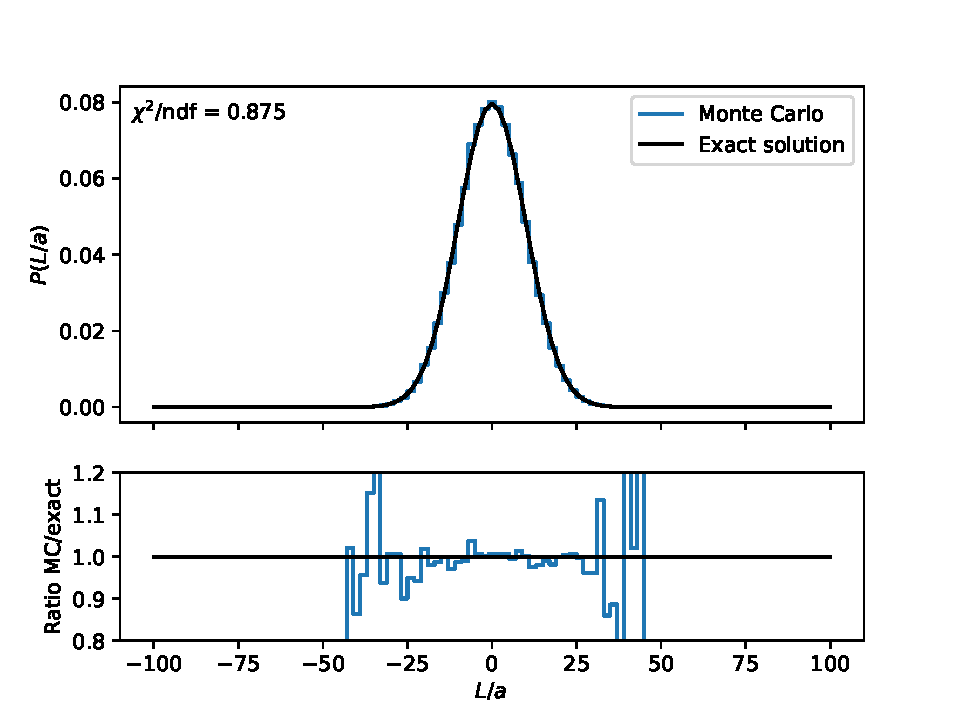
\includegraphics[width=0.8\textwidth]{demo-fig.pdf}
\end{center}
  \caption{\label{fig:demo-fig}Unbiased rubber band dimensionless length distribution. Each rubber band has $N=100$ links with $a=1$. Monte Carlo ($M=10^6$ samples) histogram is overlaid with the exact solution $P(L) = \Omega(N,n)/2^N$, the ratio plot shows good agreement (although diverging beyond the region of statistical coverage), as does the $\chi^2/$ndf of approximately unity.}
\end{figure}

\subsection*{Simulation task II: pulling with a force, reweighted}
We now introduce an external force $f$ pulling the rubber band in the positive ($+$) direction. In the previous task you constructed a Monte Carlo sampling of rubber bands unaffected (unbiased) by a force, here we will treat a biased distributed. We will do it using a \textit{reweighting technique}. This means that you do not need to resample the rubber bands, just calculate a new weight with which they enter.

\textbf{Physical idea:} Let $E$ be the energy of a single microstate. We still assume that its internal energy remain constant ($E_0$). Applying a constant force $f$ along the $+$-direction, a configuration with extension $L$ does work $-fL$, so its total energy is:
\begin{equation}
\label{eq:microstate-energy}
  E(\text{microstate with }L) = E_0 - fL.
\end{equation}
At temperature $T$, such a state has the Boltzmann weight (with $\beta = (k_B T)^{-1}$):
\begin{equation}
  w \propto e^{-\beta E} = e^{-\beta E_0}e^{\beta f L}.
\end{equation}
We already know, that for a given macrostate of length $L$, there are exactly $\Omega(L)$ corresponding microstates. Adding all their weights together, gives the macrostate weight:
\begin{equation}
  W(L) \propto \Omega(L) e^{\beta f L}.
\end{equation}
Finally, the probability to obtain a given macrostate $L$, can be found by normalizing over all possible $L$, here dummy-labelled $L'$:
\begin{equation}
  P(L) = \frac{\Omega(L) e^{\beta f L}}{\sum_{L'} \Omega(L') e^{\beta f L'}}.
\end{equation}

\begin{itemize}
  \item Extend your \texttt{RubberBand} class with a method that calculates the Boltzmann weight of a given microstate when a force $f$ is applied:
  \[
    w(\text{microstate}) = e^{\beta f L}, \qquad \beta = \frac{1}{k_B T}.
  \]
  Here $L$ is the total length calculated by your method from Task I. Hint: Work in units where $k_B = 1$, and start with $T = 1$ such that $\beta = 1$.
  \item Generate a large ensemble of microstates (still unbiased, random $\pm$-configurations). 
  \item Construct a \textit{weighted histogram} of the $L$ distribution, where the microstate weight is used. This simulates what happens if the ensemble is pulled with force $f$.
  \item Compare your weighted histogram to the analytic result:
  \[
    P_f(L) = \frac{\Omega(N,n)\, e^{\beta f L}}{Z(f)}, \qquad 
    Z(f) = \sum_{L}\Omega(N,n)\, e^{\beta f L}.
  \]
  Here $\Omega(N,n)$ is the same combinatorial factor you used in Task I, and $n = (L/a+N)/2$ from inversion of eq. \eqref{eq:L-def}.
  \item Make a plot comparing your Monte Carlo $P_f(L)$ and the analytic $P_f(L)$ for at three small nonzero value of $f$, e.g $f = \{0.01, 0.05, 0.1\}$. 
  Again, plot their ratio. Be careful with $\chi^2$ since it is poorly defined for reweighted samples. I recommend skipping it here.
  \item Try three larger values, e.g. $f = \{0.1, 0.5, 1.0\}$. Do you still see ok performance? Why not? Diagnose your reweighting by calculating the number of effective samples:
  \[\mu_\text{eff} = \frac{1}{\sum_i \tilde{w}^2_i}\text{ with: } \tilde{w}_i = \frac{w_i}{\sum_j w_j.}\]
  Plot $\mu_\text{eff}/M$ as function of the force. When would you expect reweighting to start struggling?
\end{itemize}

\subsection*{Simulation task III: pulling with a force, direct simulation}
As you saw in the previous task, reweighting works only as long as the unbiased and biased ensembles overlap sufficiently. When the force grows too large, only very few unbiased configurations contribute significant weight.
To obtain reliable results at larger $f$, you must instead generate the configurations directly from the biased distribution.

\noindent \textbf{Physical idea:} When a constant external force $f$ is applied, each link in the rubber band experiences a bias: it is more likely to point in the $+$-direction than in the $-$-direction.
From the Boltzmann factor for a single link, the probability for a link to point in the $+$-direction is:
\begin{equation}
\label{eq:pplus}
p_+(f) = \frac{w_+}{w_+ + w_-} = \frac{e^{\beta f a}}{e^{\beta f a} + e^{-\beta f a}} = \frac{1}{2}(1 + \tanh(\beta f a)), 
\end{equation}
where $\tanh$ in the last equality is the hyperbolic tangent function. Correspondingly:
\begin{equation}
  p_-(f) = 1 - p_+(f).
\end{equation}
Thus, for a given $f$ you can sample each link independently with these probabilities, instead of assigning random $\pm$ directions with equal weight.

\exercise{
Fill in the algebra needed to write the last equality in eq. \eqref{eq:pplus}. (Hint: Look up the definition of $\tanh(x)$ in terms of exponentials).
}

With that in place, we can calculate the expectation value for our upcoming ``observable'': $\langle L \rangle(f)$, the (average value) of length given a force. It is simply:
\begin{eqnarray}
\label{eq:full-analytic}
  \langle L \rangle(f) & = a \cdot (\text{number of links in the}+\text{-direction}-\text{number of links in the}-\text{-direction}) \\ 
  & = aN(p_+ - p_-) = Na (2p_+ - 1) = Na\tanh(\beta f a).
\end{eqnarray}
In the small-force limit $\beta f a \ll 1$, we can Taylor expand $\tanh(\beta f a) \approx \beta f a$ such that:
\begin{equation}
\label{eq:hooke-approximation}
  \langle L \rangle(f) \approx \frac{Na^2}{k_B T}f,
\end{equation}
matching exactly what was found in eq. \eqref{eq:hookes-law}. The task is now to Monte Carlo simulate a large number of biased states and compare the results to theory.

\begin{itemize}
  \item Change the constructor of \texttt{RubberBand} adding optional arguments \texttt{kBT} and \texttt{force}. Now your \texttt{Link} directions should be sampled from the biased distribution instead of unbiased\footnote{Note that eq. \eqref{eq:pplus} directly gives a probability to be $+$ as function of the given parameters. Instead of being $+$ with $p=0.5$, the link should now be $+$ with probability $p_+(f)$.}.
  \item Generate a large ensemble (not as large as before, $M=5000$ should be enough) of rubber bands at several values of $f$ using this biased sampling. For each $f$, compute the mean extension:
  \[\langle L \rangle(f) = \frac{1}{M}\sum^M_i L_i(f),\]
  and its standard deviation.
  \item Plot $\langle L \rangle$ as a function of $f \in [0,2.5]$. Compare to the analytic results derived in eq. \eqref{eq:full-analytic}.
  \item Use your simulation to extract the effective spring constant $k_\text{eff}$ by fitting $\langle L \rangle$ vs. $f$ in the linear region. Does $k_\text{eff}$ agree with the theoretical value $k_B T/(Na^2)$? (you could use the error from the fit to make the agreement quantitative, but you don't have to)
  \item Finally: what happens when $f$ becomes large? Show that the distribution $P_f(L)$ becomes narrow and strongly shifted, and that the linear approximation (Hooke's law) breaks down. You can do this by plotting the standard deviation as a shaded area around the mean, and plot the linear fit along with it.
\end{itemize}

One of the final points, that the distribution becomes more narrow as the force increases, may not be obvious.
However, we can also show this analytically. Recall the calculation of the average in eq.~\eqref{eq:full-analytic}.
We can calculate the variance of the $L$ distribution as the force increases using similar reasoning.
Since $L = a(2n - N)$ and $n$ follows a binomial distribution\footnote{
The variance of a binomial distribution with $N$ trials and probability $p$ of success is $\sigma^2 = Np(1-p)$.
}, we obtain\footnote{
Variance is invariant under constant shifts and scales quadratically under rescaling.
}:
\begin{equation}
  \sigma^2(L) = \sigma^2 \left(a(2n - N)\right)
  = 4a^2 \sigma^2(n)
  = 4a^2N p_+(1-p_+).
\end{equation}
Inserting $p_+$ from eq.~\eqref{eq:pplus} and applying a bit of algebra gives:
\begin{equation}
\label{eq:sigma2l}
  \sigma^2(L) = \frac{a^2 N}{\cosh^2(\beta f a)}.
\end{equation}
As the force grows, $\cosh(\beta f a)$ increases and $\sigma^2(L)$ decreases: the chain becomes increasingly aligned with the force.

\exercise{
  Complete the derivation of eq.\eqref{eq:sigma2l}, using the hints given. Remember to look in the footnotes for the variance of a binomial and properties of variance, if you don't know these by heart.
}

For someone used to handling statistical estimators, this may be an easy derivation.
Others can note that with Monte Carlo, it was no more difficult to calculate the variance than the mean.
This is one of the true powers of Monte Carlo: once your simulation is set up, you can compute any observable from its output.

\subsection*{Simulation task IV: Nearest-neighbor corrections}
The first three tasks establish a complete simulation of the entropic spring and its response to an external force.
Completing these tasks carefully, with proper validation and discussion, constitutes a full project.

Task IV extends the model by introducing correlations between neighboring links. It builds directly on the techniques from the workshop (reweighting and effective sample size) and is the natural next step if you finish Tasks I–III comfortably.

You are encouraged to attempt Task IV if time allows. It is not required for passing the course, but it is an excellent opportunity to deepen your understanding of statistical mechanics and Monte Carlo methods.

Real polymers are not made up of completely freely flipping links. Neighboring links tend to align with each other, giving the polymer a stiffness. We can model this by correcting the microstate energy of eq. \eqref{eq:microstate-energy} by a term penalizing bends. To do so, we introduce a notation for the links. Let each link be denoted by $s_i$, where:
\begin{equation}
 s_i = 
 \begin{cases} 
   1 & \text{when pointing in the }+\text{ direction}\\
   -1 & \text{when pointing in the }-\text{ direction}.
 \end{cases}
\end{equation}
Let neighboring links ($i$ and $i+1$) interact by adding a term to the energy $-Js_is_{i+1}$. $J$ is the ``stiffness'', which here is $\geq 0$. A large $J$ means that aligned neighboring links are energetically favored, while oppositely oriented links are penalized. The corrected version of the microstate energy now reads:
\begin{equation}
\label{eq:ising-hamiltonian}
  E(\{s_i\}) = E_0 - fL- J\sum^{N-1}_{i=1}s_i s_{i+1}\text{, with: } L = a\sum^N_{i=1} s_i.
\end{equation}
The Boltzmann weight of such a state is:
\begin{equation}
  w = e^{-\beta E} \propto e^{\beta (fL + J\sum^{N-1}_{i=1}s_i s_{i+1})}.
\end{equation}
This means that we can reweight our microstates to ones with correlations. In the following we will generate samples at fixed $f$ with direct sampling (like you implemented in the previous task) and reweight only in $J$. The part of the weight including the force therefore drops out. From an implementation point of view, this is structurally identical to Task II: only the definition of the weight changes.

\begin{itemize}
  \item Start by revisiting your \texttt{Link} class, and ensure that you are storing the links directions as $-1$ or $+1$ in the negative and positive directions respectively, to mirror the definition of $s_i$.
  \item Make a derived class of your \texttt{RubberBand} class, call it e.g. \texttt{CorrelatedRubberBand}, where you override your previously implemented method for calculating the weight when a force is applied to return:
  \[w(\text{microstate}) = e^{\beta J\sum^{N-1}_{i=1}s_i s_{i+1}}.\]
  The power of a derived class with an overridden weight method is, that you can now \textit{reuse all your previous code} for analyzing reweighted samples, only replacing \texttt{RubberBand} with \texttt{CorrelatedRubberBand}.
  \item Investigate the behaviour of combining generation with fixed $f$ (either positive or negative) and changing $J$. You can plot the $L$ distribution in a few cases and compare to the theoretical curve at the same fixed $f$ but with no $J$. Show that the presence of a $J>0$ seems to enhance and slightly skew the pull regardless of the sign of $f$. What is the physical mechanism?
  \item Select a value of $f$, vary $J$ and plot $\mu_\text{eff}/M$ vs $J$. How much can we vary $J$ using reweighting? Can you think of ideas to improve our coverage?
\end{itemize}

\subsection*{Epilogue: Realistic models}
The model you have just simulated in the final task is equivalent to
the one-dimensional \textit{Ising model}, originally invented to describe magnetism in materials. In that context, each link 
$s_i = \pm 1$ represents a tiny magnetic moment (a ``spin'') that can
 point up or down, while the parameter $J$ describes how strongly
  neighboring spins prefer to align. The external force $f$ in our 
  rubber band plays exactly the same role as an external magnetic field.

In polymer physics, this simple model already captures important qualitative behavior. 
Real molecules such as DNA are not freely jointed: chemical and electrostatic interactions 
give them a \textit{bending stiffness}. Neighboring molecular segments tend to align over 
some typical distance before they bend, leading to what is called a \textbf{persistence length}. 
In our one-dimensional model, the persistence length is closely related to how long segments of 
consecutive links point in the same direction — this is the \textit{correlation length} of the model.

Analytic solutions for correlated systems like this quickly become difficult. The one-dimensional 
Ising model can still be solved exactly with advanced methods, but already in two dimensions the 
solution — found by Lars Onsager in 1944 — is a classic milestone in theoretical physics. In three 
dimensions, no exact solution is known even today.

From the computational side, however, extending the model to higher dimensions is entirely feasible.  The underlying Monte Carlo logic remains the same: generate configurations, assign weights, and compute observables as averages. Only the bookkeeping (neighbors, boundaries, and visualization) becomes more involved. Modern simulations of polymers, proteins, or magnetic materials rely on exactly these ideas, just implemented efficiently and in more complex geometries.

Looking forward, this small project has given you a foundation for exploring far richer systems: from polymers and biophysics to phase transitions and materials science. The same statistical reasoning and sampling methods scale far beyond a one-dimensional rubber band — into the models that describe the microscopic structure of our physical world.

\subsection*{What to submit?}
Readable, documented code in a merge request to the exercise project. You should clearly describe your results and the methods used. It must include at least:
\begin{itemize}
  \item \textbf{Code:}
  \begin{itemize}
    \item Classes for \texttt{Link} and \texttt{RubberBand}.
    \item Cleanly separable code for solving the different simulation tasks.
    \item Reusable code for plotting comparisons with theory with a ratio plot.
    \item Code for producing all comparison plots, reweighting plots and direct simulation plots.
    \item (Task IV only) A derived class \texttt{CorrelatedRubberBand} with a correctly implemented nearest-neighbor weight method, and demonstration of its use for reweighting in $J$.
    \item Information about how to run the code, documentation of dependencies if needed.
  \end{itemize}
  \item \textbf{Documentation:}
  \begin{itemize}
    \item A clear description of the problem (no need to go through all the theory, but an overview).
    \item Description of the theoretical curves you compare to.
    \item Clear descriptions of the use of both direct simulation and reweighted techniques.
    \item A discussion of when reweighted methods break down.
    \item (Task IV only) For the correlated case, a short discussion of how introducing a stiffness parameter $J$ affects the $L$ distribution. Include at least one example plot illustrating the change in $P(L)$ as $J$ increases, and one plot of $\mu_\text{eff}/M$ versus $J$.
    \item (Task IV only) A brief interpretation of the physical meaning of $J$, relating it to stiffness or alignment of neighboring links (no detailed derivation needed).
  \end{itemize}
\end{itemize}


\subsection*{Finished early? Stretch goals}
If you complete the core tasks ahead of time, pick one or more of the extensions below. Document what you changed and, if relevant, how it affected your results or the runtime of your code. You are also free to choose a stretch goal on your own, for example exploring the Task IV extension of the model in more detail.

\subsubsection*{Python is so slow! (optimization, \texttt{C++})}
You may have noticed that simulating a large number of rubber bands can be painfully slow in \texttt{Python}. Delegate the simulation task to \texttt{C++} and call it through an API (see the 2nd day \texttt{Python} tutorial from the beginning of the course). You should deliver:
\begin{itemize}
  \item \texttt{C++} code callable from \texttt{Python} with clean instructions for how to build and run through the API.
  \item Documentation of runtime improvements, for example number of rubber bands generated per clock time in \texttt{Python} vs. \texttt{C++}.
\end{itemize}

\subsubsection*{Animate a rubber band (visualization)}
Create a short animation of a single rubber band as the force increases, showing the random links gradually aligning with the force direction. Let ``time'' in the animation be the force, which is gradually building up. Your animation should show the individual links. You should deliver:
\begin{itemize}
  \item Runnable code to produce the animation.
  \item A \texttt{.gif} file uploaded to the gitlab.
  \item Explanation of your process and the animation in the documentation.
\end{itemize}

\begin{center}
\textbf{Happy Hacking!}
\end{center}
\end{document}
